\documentclass[xetex,14pt]{beamer}

\usefonttheme{professionalfonts}
\usefonttheme{serif}

\usepackage{xltxtra}
\usepackage{xcolor}
\usepackage{minted}
\usepackage[magyar]{babel}

% \setmainfont{Roboto}
\setmainfont{Helvetica Neue LT Pro 45 Light}
\definecolor{node-bg}{HTML}{303030}
\definecolor{node-fg}{HTML}{80BD01}

\usetheme{Rochester}
\setbeamercolor{background canvas}{bg=node-bg}
\setbeamercolor{normal text}{fg=white}
\setbeamercolor{frametitle}{fg=black}
\setbeamercolor{title}{fg=black}
\setbeamercolor{structure}{fg=node-fg}

\beamertemplatenavigationsymbolsempty

\title{Node.js backend multiplayer játékhoz}
\subtitle{SpaceGame}
\author{Dányi Bence\\\small{Konzulens: Imre Gábor}}

\begin{document}
  \frame{\titlepage}
  \begin{frame}
    \frametitle{A project}
    \begin{itemize}
      \item Többjátékos shooter, Asteroids stílusban
      \item JavaScript frontend (böngésző alapú)
      \item JavaScript backend (NodeJS alapú)
      \item WebSocket alapú kommunikáció
    \end{itemize}
  \end{frame}
  \begin{frame}
    \frametitle{Technológiák}
    \begin{itemize}
      \item Babel (fordítás)
      \item Flowtype (statikus típusosság)
      \item browserify (csomagolás)
      \item React (ui)
      \item redux (játéklogika)
    \end{itemize}
  \end{frame}
  \begin{frame}
    \frametitle{Architektúra}
    \begin{center}
      
\includegraphics[width=0.7\textwidth]{figures/app-white}
    \end{center}
  \end{frame}
  \begin{frame}
    \frametitle{Szinkronizáció}
    Probléma: azonos állapot lásson minden kliens
    \begin{itemize}
      \item Játéklogika replikálása minden kliensen
      \item Minimális kliens-szerver kommunikáció
    \end{itemize}
    \vfill
    
\includegraphics[width=\textwidth]{figures/ws-white}
  \end{frame}
  \begin{frame}
    \frametitle{Játéklogika}
    Könnyen tesztelhető, \texttt{(state, action) => state} alakú determinisztikus függvény
    \begin{itemize}
      \item \texttt{state}: perzisztens adatstruktúra
      \item determinisztikus: azonos bemenetre mindig azonos kimenet
      \item környezet független (bárhol futhat)
    \end{itemize}
  \end{frame}
  \begin{frame}
    \frametitle{Játéklogika, folytatás}
    Szimuláció két lépésben:
    \begin{itemize}
      \item fizikai szimuláció az „eltelt” időről
      \item az akció idejét a szerver határozza meg
      \item az akció végrehajtása (fegyver elsütése, stb.)
    \end{itemize}
    \vfill
    A darabosság elkerülésére a kliens egy „előre szimulált” valósidejű állapotot lát.
  \end{frame}
  \begin{frame}
    \frametitle{Fizikai szimuláció}
    \begin{itemize}
      \item Diszkrét időszimuláció
      \item Minden testre erő + forgatónyomaték hat
      \item Minden időszeletben egyenletesen gyorsuló mozgás
    \end{itemize}
    „Jó” közelítése egy bonyolult differenciálegyenletnek.
  \end{frame}
  \begin{frame}
    \frametitle{Az elkészült játék}
    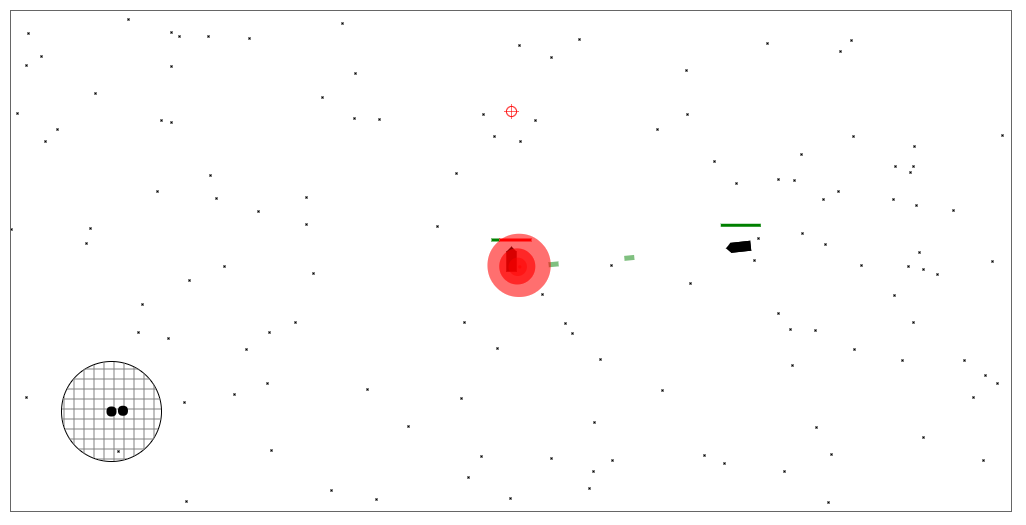
\includegraphics[width=\textwidth]{figures/screenshot}
  \end{frame}
  \begin{frame}
    \frametitle{Köszönöm a figyelmet!}
    \begin{itemize}
      \item https://github.com/madbence/spacegame
      \item https://spacegame.danyi.me
      \item Kérdések?
    \end{itemize}
  \end{frame}
% etc
\end{document}
